\documentclass[a4paper]{article}

\usepackage[ngerman]{babel}
\usepackage{amsmath}
\usepackage[ansinew]{inputenc}
\usepackage[section]{placeins}
\usepackage{geometry}
\geometry{a4paper,left=3cm,right=2cm, top=2cm, bottom=2cm}
\usepackage{color}
\usepackage{transparent}
\usepackage{graphicx}

\usepackage{float}
\graphicspath{{Figures/}}

\usepackage{epstopdf}
%-------------------
\newenvironment{boxed2}
    {\begin{center}
    \begin{tabular}{|p{0.9\textwidth}|}
    \hline
    }
    { 
    \\\hline
    \end{tabular} 
    \end{center}
    }

\def\msquare{\mathord{\scalerel*{\Box}{gX}}}
\setlength{\parindent}{0pt}



%----------
\setlength{\parindent}{0pt}

\begin{document}
\pagestyle{empty} \enlargethispage*{25cm}\samepage{

\vspace*{-3cm}
\begin{center}
\begin{minipage}[!h]{18cm}
\hspace*{-0.9cm}
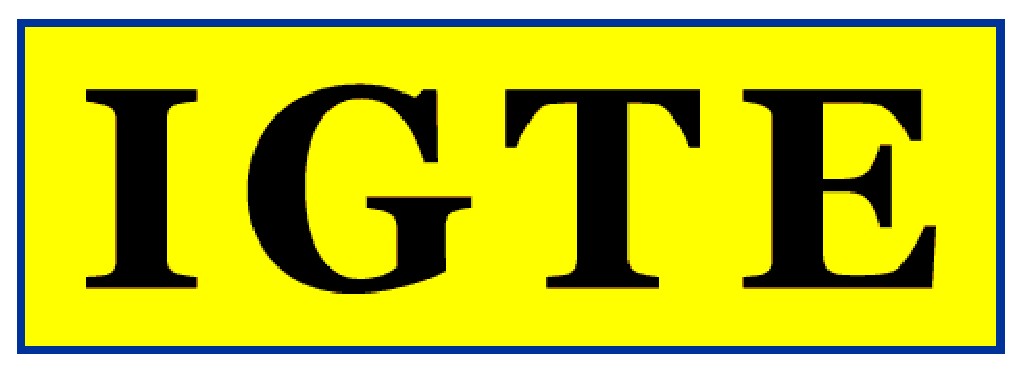
\includegraphics[width=3.3cm]{./figures/igte_logo}
\begin{tabular}{p{10cm}}
\vspace{1cm}
\centering{
\Large Institut f\"ur Grundlagen und Theorie der
Elektrotechnik \\
Technische Universit\"at Graz\\
~\\
~\\}
\end{tabular}

\includegraphics[width=3.3cm]{./figures/TUG_logo}
\end{minipage}
		\Large
		\textbf{Grundlagen der Elektrotechnik WS 22/23} \\
		\textbf{INSERT-EX-NUM. \"Ubungszettel \\ Gruppe INSERT-GROUP}\\
		INSERT-EX-NAME
	\end{center}}
	
	\vspace*{1cm}
\begin{boxed2}
\begin{center}
 \textbf{Infobox zur Netzwerkanalyse}\\
Systeme zu beschreiben und zu analysieren z"ahlt zu den essenziellen Aufgaben eines Ingenieurs. Daf"ur muss zuerst ein Modell erstellt werden, das dieses System m"oglichst gut beschreibt, um anhand dieses Modells Berechnungen anstellen zu k"onnen. In vergangenen "Ubungen haben Sie schon so ein Modell kennengelernt: Der Ohm'sche Widerstand, der ein Bauteil darstellt, an dem ein linearer Zusammenhang zwischen Strom und Spannung herrscht.  Der Widerstand wird unter anderem daf"ur verwendet, Verbraucher zu modellieren, z. B. als Modell f"ur einen Heizstrahler.\\
Um nun komplexere Systeme aus Widerst"anden betrachten zu k"onnen, lernen Sie mit diesem "Ubungsblatt den Umgang mit den Kirchhoff'schen Regeln, die als Grundlage f"ur die Netzwerkanalyse dienen. Auch das Erkennen und Verstehen von Strukturen wie den Spannungsteiler oder den Stromteiler soll hier gefestigt werden, da Sie diese in ihrem gesamten Studium und dar"uber hinaus begleiten werden.
\end{center}
\end{boxed2}
	
INSERT-TASKS

\end{document} 
